\documentclass{article}
\usepackage[margin=0.5in]{geometry}
\usepackage[export]{adjustbox}
\usepackage{indentfirst}
\renewcommand{\familydefault}{\sfdefault}
\setlength{\parindent}{1cm}
\title{Andres Ponce}

\begin{document}
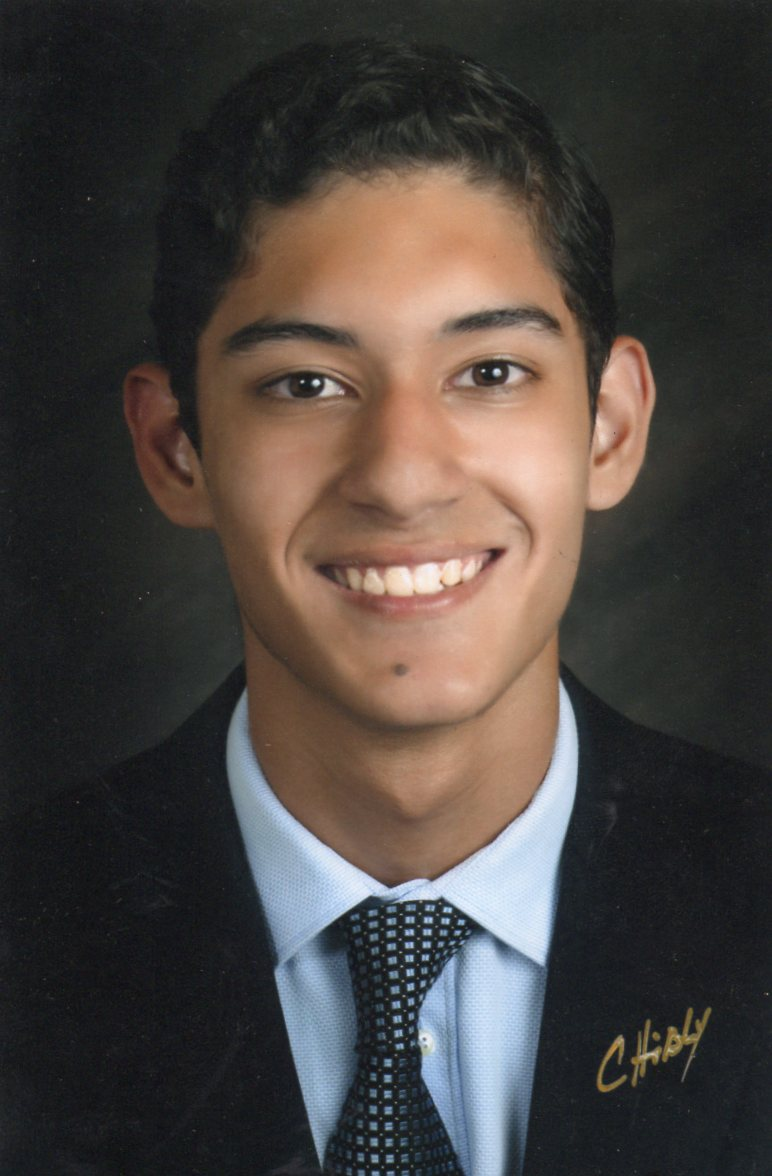
\includegraphics[width=2in,height=2in,right]{images/foto.jpg}
\begin{center}
\Huge Andres Ponce
\end{center}

My name is Andres Ponce, I was born in Honduras, a small country
in Central America. Since I was a kid, learning new things has 
always been a part of me. As a young boy I would spend hours
in my school library reading about various topics, and this passion
is something I have proudly maintained all the way into adulthood. 
I was fortunate enough to attend a school where all the instruction
was carried out in English; this has opened various opportunities 
of communication and relations while living abroad. 

The opportunity such an education afforded me filled my mind with 
dreams of going abroad to study, especialy considering the 
situtation in my country. I tried to consider as many options 
as I could, pondering what could be done given my  circumstances. 
My brother had come to Taiwan two years before I graduated high school,
and given how positively he referred to Taiwan, my parents encouraged
me to apply to the Taiwan scholarship offered by the Taiwanese embassy 
in my country. 

In August of 2016, I landed in Taiwan not knowing a word of Chinese 
and in a foreign culture. From 2016 to 2017, my year was spent studying
Chinese at National Taiwan Normal University in Taipei, and that year 
has proven so helpful while doing my undergraduate degree: not only for
granting the ability more comfortably, but also allowing the experience
of learning a beautiful language such as Chinese.  

When my year of studying Chinese was almost over, after applying to 
several universities in Taiwan, I decided that I would pursue my 
undergraduate degree in National Chiao Tung University, in the 
highly regarded Computer Science department. The experience has been
highly rewarding, letting me gain insight into areas of computing 
that I had previously never imagined were possible. Courses that range
from databases to compilers and artificial intelligence show the great
amount of variety within the field, as well as the amount of potential
for learning and self-improvement in these areas.

\end{document}
